\chapter{El FN dentro del sistema político francés}

Una vez establecido, de manera general, el caracter NAP del Front National debemos estudiar de manera un poco más detallada a este partido. Para ello presento breves resúmenes del sistema político francés, así como de la historia del partido. Así podremos estar en mejores condiciones para entender dónde y cómo participa políticamente el FN y cuál ha sido su desarrollo general. 

\section{Recuento del sistema político}

Los sistemas políticos tradicionales son el presidencialismo y el parlamentarismo \parencites[12]{Carpizo04}[39]{Veser99}. Mientras que en el primero el poder se concentra en un presidente, tradicionalmente electo por sufragio universal para un periodo fijo, en el segundo es un parlamento el depositario de la soberanía popular, por lo que el gobierno depende de la confianza de dicha asamblea \parencite[52]{Linz90}. Sin embargo, estos no son los únicos dos sistemas políticos de gobierno. Existe también el llamado \textit{régimen semipresidencial}. Este término fue popularizado por el sociólogo francés Maurice Duverger y tradicionalmente se emplea para todos aquellos regímenes híbridos que no son sistemas totalmente  presidenciales ni parlamentarios \parencites{Veser99}[7]{Carpizo04}[52]{Linz90}. De entre estos regímenes semipresidenciales, el más conocido es la actual V\textsuperscript{ta} República francesa \parencite[7]{Carpizo04}.\\

\subsection{Semipresidencialismo francés}

Para Duverger, un régimen semipresidencial como el francés tiene tres componentes principales \parencite[42]{Veser99}:

\begin{enumerate}
\item El presidente de la república es electo por sufragio universal;
\item posee considerables poderes;
\item tiene frente a él, no obstante, un primer ministro y ministros que poseen poderes ejecutivos y gubernamentales y pueden permanecer en el poder solo si el parlamento no muestra su oposición a ellos.
\end{enumerate}

Las primeras dos componentes tienen un caracter marcadamente presidencial. Sin embargo, el tercer punto es un contrapeso parlamentario que hace que el régimen no sea del todo presidencial. En general, los tres puntos se reflejan en la actual constitución, promulgada el 4 de octubre de 1958 y que instauró la V\textsuperscript{ta} República. El primero, empero, no fue totalmente concretado sino hasta el referéndum plebiscitario de 1962 que estableció el sufragio universal directo para la elección a la presidencia de la república.\footnote{Ya desde el texto original de 1958 la Asamblea nacional era electa de manera directa por la ciudadanía, pero la primera elección presidencial de la V\textsuperscript{ta} República fue mediante un colegio electoral.} Por otro lado, como sugeriría el segundo punto de Duverger, el presidente es la piedra angular del régimen francés \parencite[secc. III]{AN17a}; es el Jefe del Estado: vela por el respeto a la Constitución, asegura el funcionamiento regular de los poderes públicos así como la continuidad del Estado, es el garante de la independencia nacional, de la integridad del territorio y del respeto de los tratados \parencite[art. V]{ConstFr}. Algunos de los poderes más importantes del presidente francés son los siguientes \parencites[secc. III]{AN17a}{ViePublique}: 

\begin{itemize}
\item Nombra al Primer Ministro y acepta su dimisión. 
\item Puede disolver la Asamblea Nacional. 
\item En casos extremos puede tomar poderes extraordinarios. 
\item Puede someter a referéndum ciertos proyectos de ley. 
\item Tiene dos áreas de predominancia: 
		\begin{itemize}
		\item La Defensa, pues es comandante supremo de las fuerzas armadas y quien decide sobre el uso de la fuerza nuclear. 
		\item Las Relaciones Exteriores, pues es quien negocia y ratifica los tratados, acredita los embajadores franceses ante otros Estados y es frente a quien se acreditan los embajadores ante Francia.
		\end{itemize}
\end{itemize}

\begin{figure}[h]
	\centering
	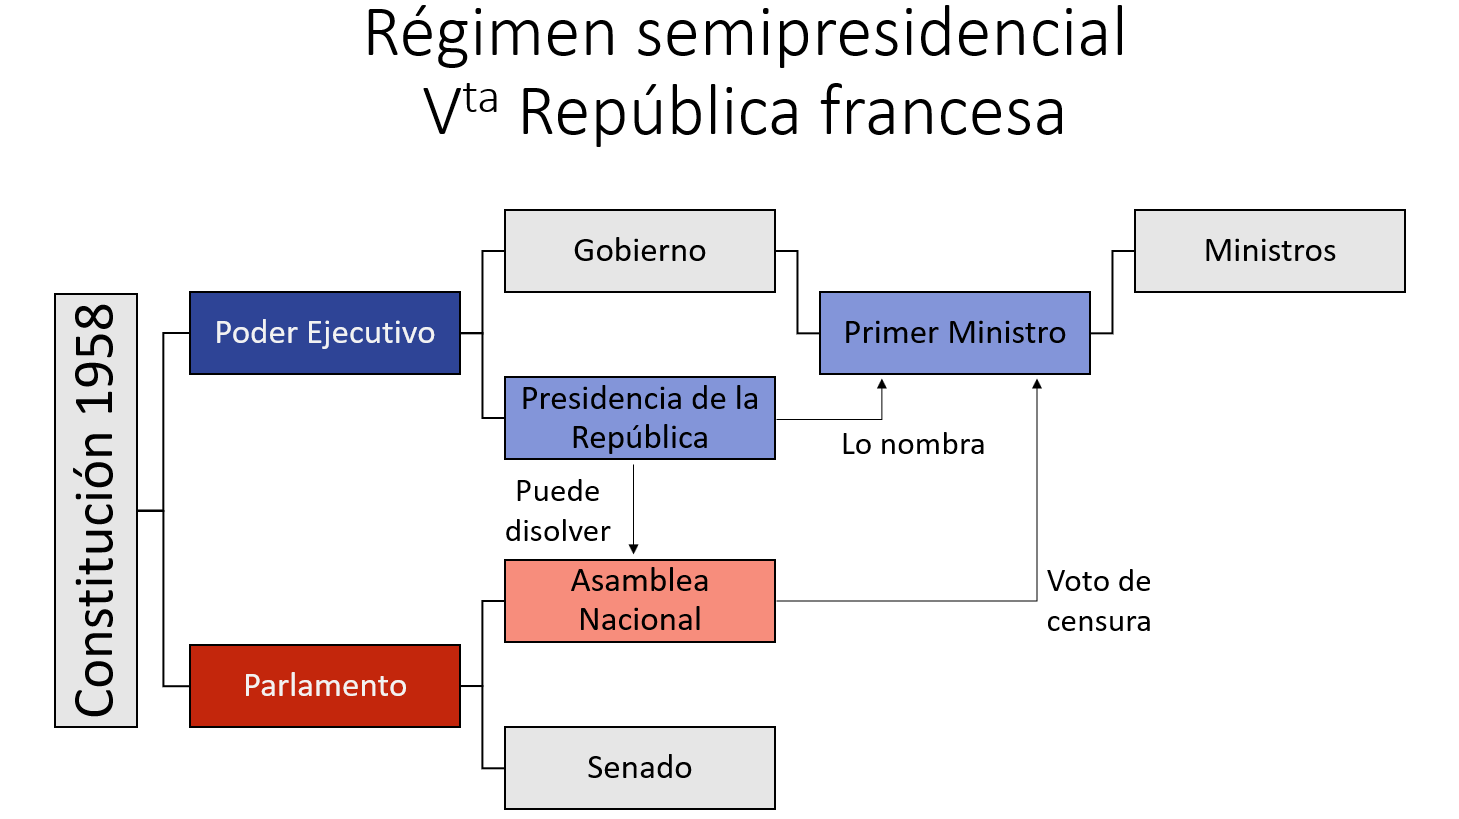
\includegraphics[scale=0.25]{Figs/FN_Francia/RegSemiPresFrVta}
	\caption{Esquema del régimen semipresidencial francés de la V\textsuperscript{ta} República. Los poderes ejecutivo--- Presidencia de la República y Gobierno--- y legislativo--- Parlamento bicameral--- están separados. El Presidente nombra al Primer Ministro, quien forma un Gobierno que depende de la confianza de la Asamblea Nacional, misma que puede ser disuelta por el Presidente. Fuente: elaboración propia.}
	\label{fig:Regimen_Semipresidencial_VRepFr}	
\end{figure}

Sin embargo, a diferencia de lo que sucede en un régimen estrictamente presidencial, el presidente no es el Jefe de Gobierno. De hecho, el poder ejecutivo en Francia está divido entre la Presidencia y el Gobierno. El Primer Ministro es el Jefe de Gobierno y es este Gobierno formado por los ministros de las diferentes carteras el que determina y conduce la política, dispone de la administración pública y asegura la ejecución de las leyes \parencite[título III]{ConstFr}. Más aún, y en sincronía con el tercer componente de Duverger, el Gobierno es responsable frente a un Parlamento bicameral, compuesto por una Asamblea nacional y un Senado. Sin embargo, esta división no es totalmente equitativa pues es solamente la Asamblea nacional quien puede remover al Gobierno.\footnote{Existen tres mecanismos por los cuales la Asamblea nacional puede obligar a un Gobierno a renunciar. El primero es usualmente llamado \textit{voto de confianza} y se da cuando el Primer Ministro somete su programa o alguna política general a la confianza de la Asamblea que vota y si la niega, el Gobierno debe renunciar. La segunda es el \textit{voto de censura} que se da por iniciativa de la Asamblea y en caso de aprobarse el Gobierno cae. Finalmente el Gobierno, bajo ciertas circunstancias, puede condicionar su responsabilidad a una iniciativa particular: si la Asamblea no está de acuerdo con el proyecto debe censurar al Gobierno y destituirlo o de lo contrario el texto propuesto es aprobado automáticamente \parencite{AN17c}.} Esta estructura general puede verse en el esquema de la \textbf{Figura \ref{fig:Regimen_Semipresidencial_VRepFr}}.\\ 

¿Qué implicaciones tiene esta configuración legal? Como bien apunta \textcite[7-8]{Carpizo04}, el régimen semipresidencial francés en la práctica es un régimen de alternancias entre un sistema (casi) presidencial y uno (casi) parlamentario. Cuál de estos subsistemas imperará depende de lo que \textcite[70]{Marrani09} llama la sincronía dentro del ejecutivo y que depende de la configuración política de las tres instituciones resaltadas en la \textbf{Figura \ref{fig:Regimen_Semipresidencial_VRepFr}}: la Presidencia, la Asamblea Nacional y, por tanto, el(la) Primer(a) Ministro(a).\footnote{Hasta el momento solo ha habido una mujer en el cargo, Édith Cresson (1991-1992).}\\ 

Recordemos que el Presidente es quien nombra al Primer Ministro. Cuando el Presidente logra tener de su lado a la mayoría de la Asamblea nacional, este puede nombrar a quien quiera sin temor de que la Asamblea vaya a destituirlo. A pesar de que formalmente el Primer Ministro es quien gobierna, en la práctica este le debe deferencia al Presidente y se convierte solo en un facilitador de su política. Esta es la situación donde hay una sincronía al interior del ejecutivo y el sistema es marcadamente presidencial. Se da lo que \citeauthor{Marrani09} llama \textit{fait majoritaire} y que podríamos designar como el funcionamiento bajo mayoría presidencial. Sin embargo, cabe la posibilidad de que la Asamblea nacional tenga una mayoría que se oponga al Jefe de Estado. En este caso, conocido como \textit{cohabitation}, el Presidente ya no puede nombrar a quien quiera. Debe nombrar a alguien que sea apoyado por la mayoría opositora de la Asamblea.\footnote{El Primer Ministro, a diferencia de lo que sucede en un sistema puramente parlamentario, no precisa ser miembro del Parlamento; por el contrario, existe una incompatibilidad constitucional entre la función gubernamental y el mandato parlamentario \parencite[art. 23]{ConstFr}. Han habido Primeros Ministros que no eran diputados de la Asamblea y, cuando un diputado es nombrado ministro, este debe cesar sus funciones y su suplente lo reemplaza en la Asamblea.} Se da una falta de sincronización al interior del ejecutivo y el Presidente debe cohabitar con un Jefe de Gobierno políticamente opuesto a él. Aquí es cuando estamos en un subsistema de corte parlamentario pues es la mayoría parlamentaria la que gobierna y, salvo en sus dominios de predominancia, los poderes del Presidente se ven fuertemente reducidos.\footnote{Su poder de veto, que no había mencionado, permanece. Sin embargo, el poder de veto en la práctica no es tan relevante como los otros puesto que en situación de mayoría presidencial no es usualmente necesario, mientras que en periodo de cohabitación es más un mecanismo de oposición legislativa que la mayoría de la Asamblea puede superar. El Presidente también conserva su poder de disolución, pero esta es una herramienta riesgosa y costosa políticamente.} En la historia de Francia han existido tres cohabitaciones: Miterrand-Chirac (1986-1988), Miterrand-Balladur (1993-1995) y Chirac-Jospin (1997-2002).\footnote{Han habido también otros periodos en los que formalmente el Primer Ministro no pertenece al mismo partido político que el Presidente pero que sí forma parte de su mayoría presidencial, por lo que no podríamos llamarlos cohabitación. Estos han sido los cuatro gobiernos bajo la presidencia de Giscard d'Estaing--- el primero de Chirac (1974-1976) y los tres de Barre (1976-1977,1977-1978,1978-1981)--- así como los dos gobiernos de Philippe bajo la presidencia de Macron.}\\

Una vez establecido el panorama general del sistema de gobierno en Francia, resulta pertinente hacer referencia a la división territorial del país galo. 

\subsection{División territorial}

De acuerdo con el artículo 72 de la Constitución francesa, 

\begin{quote}
Las colectividades territoriales de la República son las comunas, los departamentos, las regiones, las colectividades con estatus particular y las colectividades de ultramar...
\end{quote}

\begin{figure}[h]
	\centering
	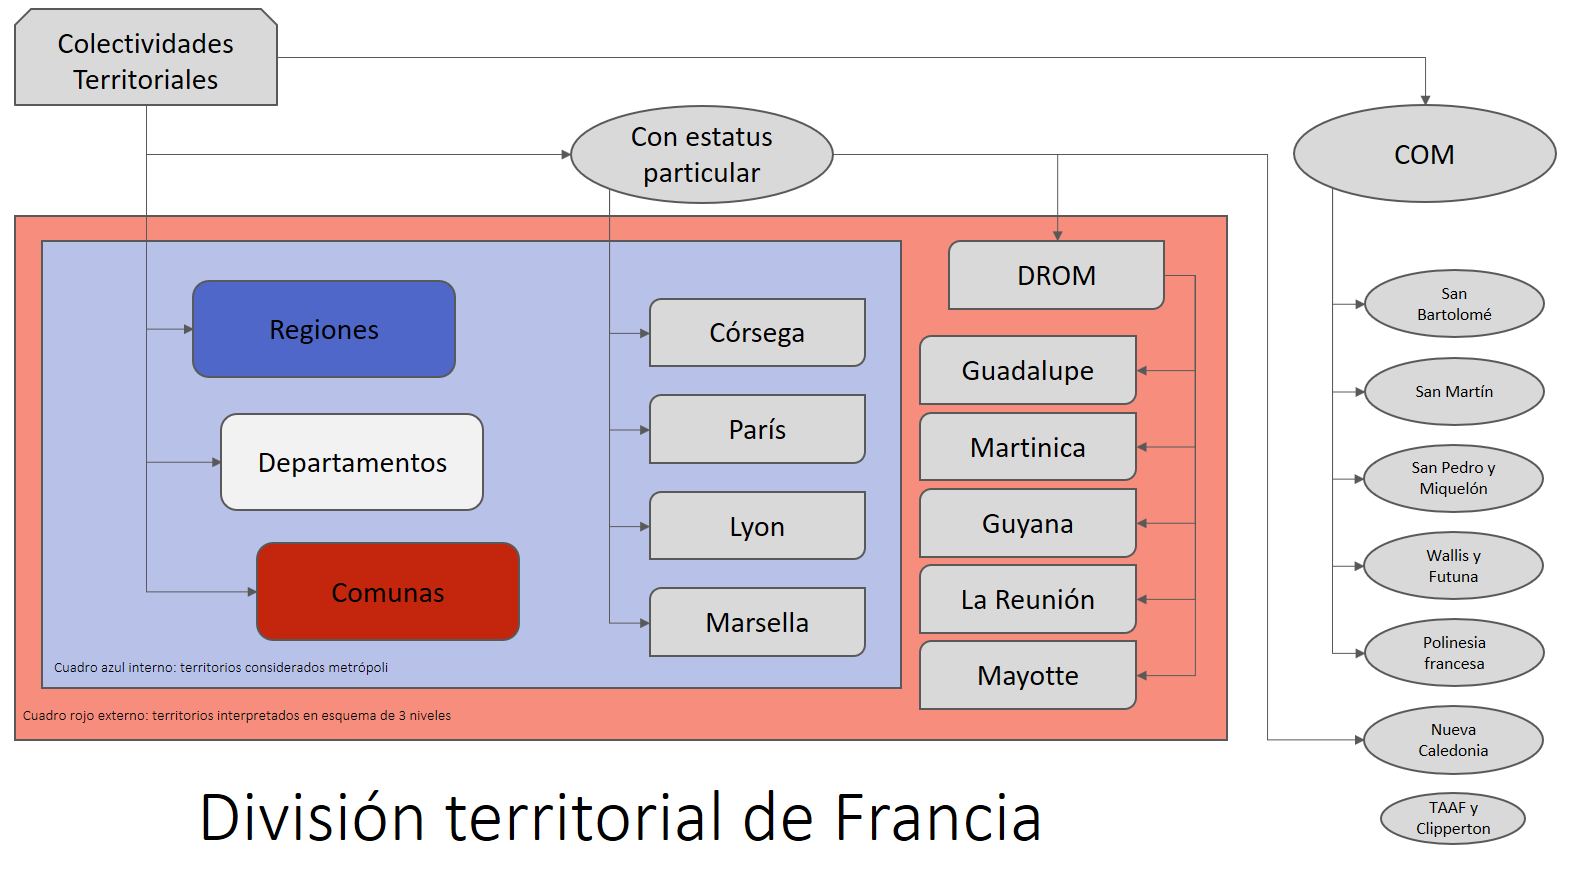
\includegraphics[scale=0.25]{Figs/FN_Francia/Div_Terr_Fr_v2}
	\caption{Esquema de la división territorial francesa. Fuente: elaboración propia a partir de \textcite{AN17b}.}
	\label{fig:Div_Terr_Fr}	
\end{figure}

Esta estructura general, puede verse en la \textbf{Figura \ref{fig:Div_Terr_Fr}}. Los primeros tres tipos de colectividades territoriales son los más usuales y se refieren a los 3 niveles de administración. El artículo después refiere la existencia de otros dos tipos de colectividades territoriales: las que tienen estatus particular y las de ultramar. No debe pensarse, sin embargo, que estas últimas son todas aquellas que no pertenecen a la metrópoli, identificada en la \textbf{Figura \ref{fig:Div_Terr_Fr}} mediante el recuadro azul interno.\footnote{La metrópoli incluye el territorio continental de Francia--- coloquialmente conocido como el Hexágono, por su forma--- y la isla de Córsega.} Más bien se refieren a 5 territorios específicos conocidos en Francia como \textit{Collectivités d'outre-mer} (COM): San Bartolomé, San Martín, San Pedro y Miquelón, Wallis y Futuna, así como la Polinesia francesa. Existen otros territorios del ultramar francés diferentes a las COM. Hay territorios no habitados: la Isla de Clipperton y los Territorios australes y antárticos franceses (TAAF). Encontramos también a la Nueva Caledonia como una colectividad sui generis. Finalmente, existen otros 5 territorios de ultramar que son colectividades territoriales con estatus especial, los \textit{Départements et Régions d'outre-mer} (DROM): Guadalupe, Martinica, Guyana, Reunión y Mayotte. Estos 5 DROM y otros 4 territorios en la metrópoli que también son colectividades con estatus especial--- Córsega, París, Lyon y Marsella--- usualmente son considerados dentro del sistema de 3 niveles, a pesar de las particularidades de cada uno. Así pues, el recuadro rojo externo de la \textbf{Figura \ref{fig:Div_Terr_Fr}} identifica a todas las colectividades territoriales que se interpretan bajo el esquema de 3 niveles. Estos tienen las siguientes características generales \parencite{AN17b}: 

\begin{enumerate}
\item \textbf{Comunas} \\ 
Son el nivel más cercano a los ciudadanos. Existen desde 1789 cuando remplazaron a las parroquias. Existen en Francia alrededor de 36,000, aunque año con año el número varía pues las comunas pueden fusionarse o separarse. Sus principales áreas de competencia son el urbanismo, la vivienda y el ambiente. Se gobiernan principalmente mediante un concejo municipal elegido popularmente y un \textit{maire} designado por dicho concejo.

\item \textbf{Departamentos}\\ 
El segundo nivel también fue creado en 1789. Hasta el 31 de diciembre de 2017, existían 101 departamentos, de los cuales 96 formaban la metrópoli y los otros 5 son DROM. A partir del  1ro de enero de 2018 los dos departamentos de Córsega fueron sustituidos por una colectividad única, por lo que ahora hay 100 departamentos. Tienen dos dominios de responsabilidad: la acción social y el manejo de los espacios.\footnote{Estos términos incluyen, el primero, los temas relacionados con grupos vulnerables como la infancia, las personas con discapacidad o los adultos mayores, mientras que el segundo se refiere, por ejemplo, al control de puertos, aeropuertos o caminos dentro del territorio del departamento.} Se gobiernan principalmente mediante un concejo departamental elegido popularmente y un presidente designado por dicho concejo.

\item \textbf{Regiones}\\ 
Es el nivel de más reciente creación, pues fue reconocido como colectividad territorial en 1982. Hasta 2015 existieron 27 regiones, 22 en la metrópoli--- incluída Córsega--- y las 5 DROM. En 2015 hubo una reforma que agrupó algunas, por lo que las nuevas regiones son solo 18--- 13 en la metrópoli, contando Córsega, y las 5 DROM---. Las regiones están encargadas del desarrollo económico, la administración del territorio y los transportes no urbanos. Se gobiernan principalmente mediante un concejo regional elegido popularmente y un presidente designado por dicho concejo.
\end{enumerate} 

Las colectividades territoriales usualmente son de uno de los tres niveles. Por ejemplo, \textit{Villemomble} es una de las 40 comunas que conforman el departamento de \textit{Seine-Saint-Denis}. Este, a su vez, es uno de los 8 departamentos que conforman la región \textit{Île de France}. Sin embargo, las colectividades con estatus especial pueden compartir, al mismo tiempo, dos niveles. Este es el caso de París, que también se encuentra en la región Île de France pero que es tanto un departamento como una comuna dividida en \textit{arrondisements municipales}.\footnote{Nótese que uso la palabra \textit{pueden}; Marsella tiene un estatus especial pero es solamente una comuna.}\\

Una vez que he presentado un resumen general del semipresidencialismo francés y de la organización del territorio, procedo a mencionar a grandes rasgos el sistema electoral del país.

\subsection{Principales elecciones}

Con base en lo que reporta el Ministerio del Interior francés (\citetitle{InterieurElecc}), identifico cuatro categorías de elecciones francesas. 

\begin{itemize}
\item Para conformar los poderes nacionales: 
	\begin{itemize}
	\item Presidenciales. 
	\item Legislativas, para la Asamblea nacional.
	\item Senatoriales.
	\end{itemize}
	
\item Para conformar las autoridades de los 3 niveles: 
	\begin{itemize}
	\item Municipales, a nivel comuna. 
	\item Departamentales, antes conocidas como cantonales.\footnote{Antes de una reforma de 2015 las elecciones para el nivel de departamento eran conocidas como elecciones cantonales pues los consejeros se eligen en circunscripciones llamadas cantones.}
	\item Regionales.
	\end{itemize}
	
\item Supranacionales:
	\begin{itemize}
	\item Europeas, para el Parlamento europeo.
	\end{itemize}
	
\item Especiales, con diversos fines: 
	\begin{itemize}
	\item Referéndums.
	\item Comunitarias, se dan al interior de las comunas.
	\end{itemize}
\end{itemize}

De entre estas categorías, solo me concentraré en explicar un poco más las presidenciales y las legislativas por tratarse de las dos principales instituciones que determinan el funcionamiento del sistema semipresidencial francés. Ambas son elecciones de sufragio universal directo.\\

La Asamblea nacional se conforma por 577 diputados que se eligen por periodos de 5 años con reelección.\footnote{A menos que el Presidente disuelva la Asamblea antes del término de la legislatura, en cuyo caso no puede haber una nueva disolución en el año siguiente.} Se elige un diputado por circunscripción legislativa mediante un sistema de mayoría a doble vuelta. Esto significa que hay dos formas de ganar la elección: 

\begin{enumerate}
\item \textbf{En la primera vuelta}, si se obtiene la mayoría absoluta de la votación efectiva, siempre y cuando los votos recibidos representen al menos un cuarto de los electores inscritos en las listas de votación. 
\item \textbf{En la segunda vuelta}, donde basta la mayoría relativa. En caso de empate el(la) candidato(a) de mayor edad gana. 
\end{enumerate}

Pasan a la segunda vuelta todas las candidaturas que hayan obtenido un porcentaje de votación equivalente a al menos el 12.5\% de los electores inscritos en las listas de votación. Esto significa que puede haber más de dos contendientes en la segunda vuelta.\footnote{Esto da lugar a las expresiones \textit{duels}, entre dos candidaturas, y \textit{triangulaires}, entre tres. Pueden también darse cuadrangulares o segundas vueltas entre más candidatos pero son mucho menos frecuentes y, cuando suceden, tienden a haber declinaciones y alianzas.}\\

Por otro lado, tenemos la elección presidencial. En el siglo XXI han habido dos principales reformas consititucionales que han moldeado esta elección. La primera, en 2000, redujo el periodo presidencial de 7 a 5 años. Aunque esto pareciera a primera vista un control sobre el Presidente, en realidad es una reforma que refuerza al Jefe de Estado. Ahora los periodos presidenciales coinciden con los 5 años por los que son elegidos los diputados.\footnote{A menos, claro, que el propio Presidente disuelva la asamblea, cosa que no ha ocurrido desde la reforma. De hecho, solo han existido 5 disoluciones en la V\textsuperscript{ta} República, todas en el siglo XX, en 1962, 1968, 1981, 1988 y 1997.} Más aún, la elección presidencial se realiza unas semanas antes que la elección legislativa. Esto hace mucho menos probable que un presidente electo enfrente una cohabitación, pues su reciente triunfo tiende a impulsar una mayoría legislativa a su favor. Sin embargo, en 2008, se decidió limitar al Jefe del Estado prohibiendo que un presidente sirva más de dos mandatos.\\

Los presidentes también se eligen mediante mayoría a dos vueltas. Esto significa que, al igual que con los diputados, se puede ganar la elección de dos formas: 

\begin{enumerate}
\item \textbf{En la primera vuelta}, si se obtiene la mayoría absoluta de la votación efectiva.  
\item \textbf{En la segunda vuelta}, si se obtiene la mayoría absoluta de la votación efectiva. 
\end{enumerate}

Para garantizar que alguien gane la elección en la segunda vuelta, a diferencia de lo que pasa con las elecciones legislativas, solo pueden presentarse a la segunda vuelta las dos candidaturas más votadas en la primera. Sin embargo, existe un vacío legal en el caso de empate, pues el criterio de edad imperante en las elecciones legislativas no está contemplado para la elección presidencial \parencite{Parisien16}.\\

Esta sección tuvo como objetivo proveer al lector del contexto político en Francia, presentar las estructuras básicas que se intentarán aprovechar en el análisis estadístico de los datos y facilitar la lectura de la historia del Front National, pues se hacen referencia a varios de los conceptos antes presentados y que en primera instancia pueden resultar extraños. 

\section{Breve historia del Front National}

Como todo fenómeno social, el FN no ha sido un movimiento monolítico. Desde sus orígenes y hasta el día de hoy ha tenido momentos de menor y mayor éxito. Un esquema para estudiar la historia del partido, principalmente desde el punto de vista electoral, es señalar tres grandes etapas. En primer lugar, la primera década de su existencia estuvo marcada por la marginalidad política y es comúnmente llamada la \textit{traversée du désert}. En segundo lugar, a partir de los años 80 el FN irrumpe en la escena política de la mano de su líder Jean-Marie Le Pen quien, en 2002, logró alcanzar su zenit al obtener el segundo lugar en la primera vuelta presidencial de ese año. No obstante la primera década del siglo XXI estuvo marcada por el declive de la figura de Le Pen. Por ello, en 2011 comienza la más reciente etapa del partido. Jean-Marie Le Pen pasó la batuta del liderazgo a su hija Marine Le Pen quien desde entonces ha implementado una estrategia de \textit{dédiabolisation}, buscando acabar con la imagen negativa del partido, principalmente con respecto al carácter racista que caracterizó a su padre. El recuento histórico que sigue está basado primordialmente en aquellos que hacen \textcite{Hainsworth16b} y \textcite{Stockemer17}, así como en el apéndice cronológico al libro editado por \textcite{CreponEtAl15} pero algunas otras referencias se citan también.\\

\subsection{El FN del desierto (1972-1983)}

El Front National surgió como una iniciativa del movimiento \textit{Ordre Nouveau} (ON) en 1972 para unir en una plataforma electoral a distintos grupúsculos\footnote{En el sentido de grupos más bien pequeños y dispersos.} políticos extremistas como los irredentistas de la colonización francesa en Algeria, los herederos del movimiento poujadista o del régimen de Vichy, intelectuales de la \textit{Nouvelle Droite}, organizaciones juveniles como \textit{Occident} o \textit{L'\OE{}uvre Française}, revisionistas del Holocausto, monarquistas, entre otros. Jean-Marie Le Pen fue elegido presidente del partido, en parte por ser una figura relativamente conocida--- se había convertido en el diputado más joven en 1956 como parte del movimiento de Poujade y había sido el coordinador de campaña de Tixier-Vignancour en 1965--- y en parte por, irónicamente, ser visto como un moderado.\\ 

Durante los años siguientes, sin embargo, el nuevo partido hiló una serie de fracasos electorales en las elecciones legislativas de 1973, las presidenciales de 1974, las legislativas de 1978 y, de manera más particular, en las presidenciales de 1981, en las cuales Le Pen no logró las firmas necesarias para participar.\footnote{En Francia, para que una persona se pueda presentar como candidata en las elecciones presidenciales requiere 500 apadrinamientos de parte de representantes electos como pueden ser alcaldes o legisladores.} Los problemas no se limitaron a las urnas. Ya desde 1973 la multiplicidad de facciones hizo que el partido se debilitara. Después de un mitin llamado \textit{Alto a la inmigración salvaje} miembros de ON se enfrentaron en una batalla campal violenta con miembros de la Liga Comunista por lo que el movimiento fue proscrito. Esto le permitió a Le Pen tomar mayor control del partido, pero también hizo surgir en 1974 a un nuevo partido fundado por miembros de ON, el PFN(\textit{Parti des Forces Nouvelles}). En 1976 Le Pen sobrevivió a un intento de asesinato, pero su segundo al mando e ideólogo François Duprat fue asesinado por un coche bomba en 1978. El Front National parecía apenas sobrevivir.\\

Entonces, el partido comienza a poner en un segundo plano su carácter anticomunista para hacer mayor énfasis en la migración vinculando a los inmigrantes con los problemas de seguridad y desempleo. A inicios de los años 80, sus posturas nativistas, autoritarias y populistas empezaron a resonar en los votantes. El gobierno de Miterrand implementó varias medidas para facilitar la inmigración, reducir las prerrogativas de la policía y otorgó amnistías a casi el 14\% de los prisioneros. La población francesa no fue del todo favorable a ello. Los partidos tradicionales de derecha comenzaron a endurecer sus posturas frente a la migración y la seguridad. Esto le dio mayor legitimidad al FN pues le permitió normalizar, de cierta manera, su discurso.\\ 

A nivel local, el FN comienza a crecer en Dreux donde en las elecciones legislativas de 1981 logró obtener más de 10\% de los votos. En las elecciones municipales de 1983 Le Pen es nombrado consejero municipal del distrito 20 de París al obtener 11.26\% de los votos en la primera vuelta y 8.54\% en la segunda. Jean-Pierre Stirbois en Dreux logra incluso un mejor resultado: 16.72\% de los votos en la primera vuelta y una alianza con la derecha tradicional en la segunda vuelta lo llevan también a ser consejero municipal. El partido había atraversado un desierto político y estaba a punto de sorprender a propios y extraños.\\

\subsection{El FN Lepenista (1984-2010)}

La hora de la verdad de Le Pen, literalmente, llegó en 1984. El éxito en Dreux hizo que Le Pen fuera invitado en febrero de ese año al programa político de TV más visto en Francia entonces, \textit{L'heure de verité}. La entrevista fue todo un éxito y simbólicamente podría marcar el inicio de lo que aquí llamo la era lepenista del FN.\footnote{Las preferencias electorales del FN pasaron del 3.5\% al 7\% a la semana siguiente de la entrevista, por ejemplo \parencite[53]{Stockemer17}.} La confirmación de esta nueva etapa fue el 17 de junio de 1984. Las listas del FN lograron aproximadamente 11\% de los votos en las elecciones al Parlamento Europeo que se transformaron, gracias al sistema proporcional, en 10 eurodiputados de extracción frontista.\\ 

El FN ya no era un partido al margen del sistema político, lo que le permitió captar más liderazgos. El más importante de esos nuevos adherentes fue, sin duda, Bruno Mégret. En 1985 se unió al partido y en 1988 se conviertió en director general. La adición de Mégret demostraría ser fundamental para la consolidación del FN como un actor político relevante en Francia. A él se le atribuye la profesionalización de los cuadros y estructuras del partido así como la popularización de la retórica frontista y, en gran medida, el que en las elecciones de la segunda mitad de los 80 el FN haya obtenido alrededor del 10\% de manera consistente.\footnote{9\% en las cantonales de 1985, 10\% en las legislativas de 1986, 14\% en las presidenciales de 1988, 9\% en las legislativas de 1988, 11\% en las europeas de 1989, así como el primer alcalde frontista en 1989.} En los años 90 el FN continuó--- de la mano del populismo de Le Pen y la organización de Mégret--- creciendo en las preferencias electorales. En 1995, los candidatos del FN se convirtieron en alcaldes en tres ciudades relevantes: Toulon, Marignane y Orange. En las elecciones presidenciales de 1995, las legislativas de 1997 y las regionales de 1998 el frontismo se afianzó alrededor del 15\% de los votos.\\

Empero, los éxitos no estuvieron alejados de los escándalos. A pesar de los intentos de Mégret por encuadrar el nativismo del FN en conceptos más políticamente correctos--- que no más moderados--- como la \textit{preferencia nacional}, el antisemitismo de Le Pen y de otros miembros del FN era evidente. En varias ocasiones Le Pen fue centro de atención por sus comentarios antisemitas. Los más conocidos son quizás cuando dijo que el Holocausto era un ``pequeño detalle'' en la historia de la Segunda Guerra Mundial o cuando se burló de un ministro de nombre Michel Durafour llamándolo \textit{Monsieur Durafour Crématoire}.\footnote{La palabra \textit{four} en francés significa horno y agregó el término \textit{crématoire}, es decir, crematorio.}\\ 

Asimismo, con los éxitos también surgieron las rivalidades internas. El liderazgo de Mégret empezó a ser más evidente e incómodo para Le Pen. Ambos personajes tenían también visiones distintas sobre la estrategia del partido; por ejemplo, mientras Mégret abogaba por tejer alianzas con los partidos de la derecha tradicional, Le Pen siempre las rechazó, lo que a los seguidores de Mégret les hacía creer que en realidad no quería llegar al poder. Las tensiones fueron creciendo hasta llegar a un enfrentamiento directo entre 1998 y 1999. A causa de un ataque físico de Le Pen contra una candidata socialista en 1997, este estaba impedido para participar en las elecciones europeas de 1999.\footnote{Le Pen había ido a Mantes-la-Jolie a apoyar a su hija en su campaña en las legislativas de 1997. Al llegar al lugar fue recibido por manifestantes que lo increparon, llamándolo fascista. Desde que bajaron del carro, los guardaespaldas de Le Pen comenzaron a golpear a los manifestantes y eso desató una pela en la que el propio Le Pen se involucró. En un momento empujó contra un muro a la rival de su hija, la socialista Annette Peulvast-Bergeal \parencite[ver video en][seg. 49]{InaPolitique97}. Por este ataque, Le Pen fue condenado en 1998 a un año de inegilibilidad, a tres meses de prisión suspendida condicionalmente y a 5,000 francos de multa \parencite{LesEchos99}.} Mégret parecía la opción más natural para encabezar las listas del partido. Sin embargo, parafraseando a Le Pen, en el FN el único que importaba era el número uno, así que colocó a su esposa en el primer puesto en lugar de a Mégret. En diciembre de 1998, Mégret criticó a Le Pen y dijo que se había convertido en un lastre para el partido. El comité ejecutivo del partido, controlado por Le Pen, votó para expulsar a Mégret del FN. En respuesta, Mégret fundó un nuevo partido, el MNR (\textit{Mouvement National Républicain}). El cisma mégretista se llevó a casi la mitad de los miembros del FN y a su más importante operador político. Compitiendo contra el MNR, en las elecciones europeas de 1999 el frontismo sólo obtuvo el 5.7\% de los votos. No obstante, el más grande éxito de Jean-Marie Le Pen llegó apenas unos años después.\\ 

Ante una izquierda sumamente dividida--- hubo 8 candidatos de izquierda--- en una elección presidencial atípica, Le Pen sacudió a propios y extraños el 21 de abril de 2002.\footnote{La elección fue atípica no solo por la división de la izquierda sino porque en total 16 candidaturas lograron las firmas necesarias para competir, un récord en Francia. Nadie logró más de 20\% de los votos en la primera ronda, algo también inédito.} Los estrategas de los candidatos no creían lo que sus conteos rápidos les decían. A las 8 de la noche, las cadenas de televisión dieron la noticia: Jean-Marie Le Pen había quedado en segundo lugar, apenas por encima del candidato socialista, Lionel Jospin.\footnote{La diferencia fueron menos de 200 mil votos.} Del lado socialista, incredulidad, sorpresa absoluta y llanto de tristeza. Del lado del FN, también hubo incredulidad, sorpresa absoluta y llanto, pero de emoción.\footnote{En Youtube se puede encontrar un documental en francés que refleja de muy buena manera cómo se vivió esa noche electoral en Francia \parencite[por ejemplo, ver desde el min. 30]{Capo17}.} Le Pen había avanzado a la segunda vuelta presidencial. Se enfrentaría al ganador de la primera, el presidente en funciones, Jacques Chirac. Hubo fuertes llamados a unirse en torno a Chirac para evitar que ganara el candidato FN. Ante la amenaza que, para la enorme mayoría de los franceses, representaba Le Pen, Chirac fue reelecto por un amplísimo margen: 82\% vs 18\%. \\

Así pues, 2002 fue el gran éxito de Jean-Marie Le Pen, pero también el inicio del fin: era claro que la mayor parte de la población no veía en él una opción aceptable. Los resultados electorales que siguieron fueron en declive: 10\% en las europeas de 2004, 11\% en las presidenciales de 2007, 4\% en las legislativas de 2007, 6\% en las europeas de 2009. Fiel a su costumbre, Le Pen siguió mostrando su revisionismo de la Segunda Guerra Mundial al declarar en 2005 que: ``al menos en Francia, la Ocupación alemana no fue particularmente inhumana''. El partido enfrentó problemas económicos y deudas que lo obligaron a despedir a un tercio de los empleados, a cancelar su fiesta \textit{Bleu Blanc Rouge}, entre otras cosas. Era claro que Jean-Marie Le Pen ya no estaba en condiciones de liderar al Front National. Sin embargo, el líder histórico no habría de ceder el mando a cualquiera.\\

\subsection{El FN Marinista (2011-)} 
 
Cuando fue momento de pasar la batuta de su movimiento, y a pesar de que existía mucho apoyo al interior del partido para que Bruno Gollnisch--- un viejo lobo de mar del FN--- fuera el nuevo líder, Jean-Marie Le Pen decidió apoyar a su hija, Marine Le Pen.\footnote{En una elección interna anterior para el liderazgo del comité central del partido, Gollnisch había ganado mientras que Marine Le Pen había quedado en una lejana posición número 34 \parencite[265]{Williams12}.} El 16 de enero de 2011, Marine Le Pen fue elegida presidente del FN, mientras que Jean-Marie Le Pen fue nombrado presidente honorario del mismo.\\ 

La estrategia del \textit{marinisme}, en contraposición a la del \textit{lepenisme}, ha buscado \textit{desatanizar} al partido. Marine Le Pen ha querido renovar la imagen que el FN presenta a los electores. Presento dos ejemplos de estos intentos. En primer lugar, si el FN lepenista siempre fue muy vocal respecto a sus posiciones sobre los temas de prácticas y costumbres sociales o, como se les conoce en Francia, las \textit{m\oe{}urs}, bajo el liderazgo marinista, la posición oficial del FN al respecto ha cambiado. El símbolo de esta inflexión en temas sociales quizás es Florian Philippot--- vicepresidente del partido de 2012 a 2017--- quien en 2014 declaró ser gay, algo impensable en el FN lepenista.\footnote{Digo inflexión porque no ha sido un cambio total: hay cuadros que mantienen posiciones firmes en contra del aborto o los matrimonios entre personas del mismo sexo, sin embargo, la postura oficial ha sido más ambigua y ha dejado de hacer énfasis en esos temas. El lector interesado en el tema de las m\oe{}urs dentro del FN puede consultar el texto de \textcite{Crepon15}.} Por otro lado, y de manera muy particular, Marine Le Pen ha cortado al interior del partido las expresiones antisemitas y abiertamente racistas. A diferencia de lo que dijo su padre, ella ha declarado que todo el mundo sabe lo que pasó en los campos nazis, en qué condiciones sucedió y cómo representó la máxima expresión de la barbarie. De hecho, a raíz de que Jean-Marie Le Pen reafirmara en 2015 el caracter de ``pequeño detalle'' del Holocausto, Marine Le Pen empujó y consiguió la expulsión de su padre del partido.\\

Esta estrategia parece haber rendido sus frutos con el electorado. A pesar de no avanzar a la segunda vuelta en 2012, Marine Le Pen superó a su padre al obtener 18\% de los votos en la primera vuelta. En las legislativas de ese año, el FN obtuvo dos diputaciones y el 14\% de los sufragios. En 2014, el partido conquistó 11 alcaldías, sus primeros dos senadores y fue la primera fuerza política votada en las elecciones europeas con 25\%. Este crecimiento ha continuado para el partido, en 2015 el FN obtuvo el 25\% en las elecciones departamentales y el 28\% en las regionales. Finalmente, en las elecciones presidenciales de 2017, la lideresa del frontismo logró superar de nueva cuenta a su padre. Ella obtuvo 21\% de los votos de la primera vuelta, más que Jean-Marie Le Pen en 2002, lo que le permitió también avanzar a la segunda vuelta. Sin embargo en 2017, a diferencia del 2002, la presencia del FN en la segunda vuelta no fue sorpresiva sino más bien era lo esperado. Más aún, si Le Pen padre perdió dicha segunda vuelta por una diferencia de alrededor de 65 puntos porcentuales, Le Pen hija la perdió por poco más de 30. Los franceses volvieron a dejar claro que consideran, mayoritariamente, al FN como una amenaza; empero, esa percepción ha disminuido fuertemente en la era marinista del partido.\\

A pesar de estos éxitos de la estrategia de desdemonización, existen varios paralelismos con la historia de su padre. Así como Jean-Marie Le Pen tuvo a Bruno Mégret como su operador político, Marine Le Pen se apoyó en Florian Philippot para encuadrar su discurso y manejar al partido. Ambas manos derechas de los Le Pen, terminaron por salir del partido y fundar su alternativa política, aunque los motivos y circunstancias de los cismas fueron distintos. Como ya he dicho, Mégret fue expulsado después de desafiar directamente a Jean-Marie Le Pen por el liderazgo del partido. La renuncia de Philippot al FN, por el contrario, surge en medio de una introspección del partido y la búsqueda de culpables después de las elecciones de 2017.\\ 

Las elecciones presidenciales de 2017 marcaron la mayor cantidad de votos en la historia del FN. 33\% en la segunda vuelta no es un dato menor, sin embargo, para muchos significó un fracaso. Bruno Jeudy, Vanessa Schneider, Nonna Mayer y Jérôme Fourquet discutieron al respecto en el programa de televisión \textit{\textcite{CDansLAir17}}: muchas encuestas a lo largo del proceso apuntaban a que Le Pen lograría hasta 40\% de los sufragios hasta que la noche del debate entre Le Pen y Emmanuel Macron se dio un punto de inflexión. Marine Le Pen fue muy agresiva--- minando, posiblemente, el esfuerzo de desdemonización--- pero también se vio poco preparada. En un momento Macron le preguntó si ella proponía abandonar el euro y regresar al franco como moneda francesa. Su respuesta fue ambigua y muy poco clara. El debate supuso un duro golpe que le hizo perder al menos 5 puntos porcentuales de intención de voto. Más aún, la postura de abandonar el euro no fue la más popular entre el electorado e incluso dentro de buena parte de los miembros del FN. Ésta propuesta, como la mayoría del programa económico del FN, se debe a Philippot y su corriente que podríamos llamar soberanista en contraposición a la línea identitaria más dura del partido.\footnote{\textcites(Ver por ejemplo)(){Marin17}{Berteloot17}{Europe17}.} Mientras que Philippot buscaba poner más énfasis en los temas económicos y sociales, que pudieran atraer a más electores,\footnote{Particularmente de izquierda, los llamados \textit{gaucho-lepenistes}.} otros cuadros del partido buscarían resaltar la línea de inmigración y seguridad de corte más derechista. Philippot fue señalado como el culpable de la decepción. Formó una organización política interna al FN llamada \textit{Les Patriotes} y amenazó con abandonar el partido si el FN renunciaba a su posición sobre el euro. Después de las elecciones legislativas, en las que el FN logró 8 escaños pero no los 15 necesarios para convertirse en grupo parlamentario, las presiones aumentaron. Marine Le Pen le pidió elegir entre la vicepresidencia del FN y la dirección de \textit{Les Patriotes} y él respondió acusando al partido de estar cambiando de línea y regresando a un pasado absolutamente horripilante. Su destino estaba sellado: le fueron retiradas sus responsabilidades como vicepresidente y Philippot renunció al FN para convertir a \textit{Les Patriotes} en un nuevo partido político.\footnote{Ver \textcite{Galtier17, Zafimehy17}.}